\documentclass{standalone}
\usepackage{pgfplots}
\pgfplotsset{compat=newest}
\begin{document}
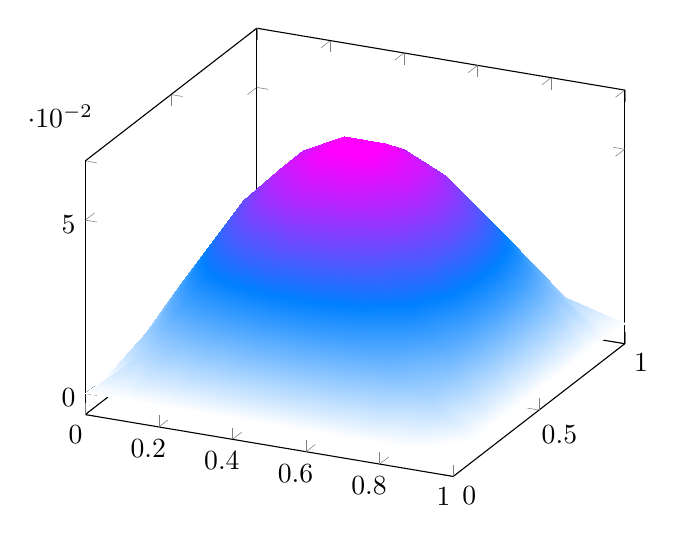
\begin{tikzpicture}
	\begin{axis}[colormap/cool]
	\addplot3[surf,samples=10,domain=0:1,
		shader=interp] 
		{x*(1-x)*y*(1-y)};
	\end{axis}
\end{tikzpicture}
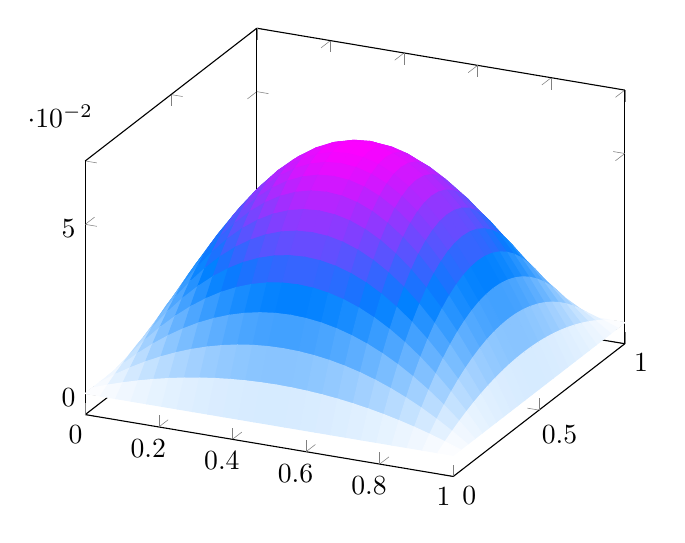
\begin{tikzpicture}
	\begin{axis}[colormap/cool]
	\addplot3[surf,samples=25,domain=0:1,
		shader=flat] 
		{x*(1-x)*y*(1-y)};
	\end{axis}
\end{tikzpicture}
\end{document}
